\documentclass[12pt]{article}
\usepackage[utf8]{inputenc}
\usepackage{geometry}
\usepackage{graphicx}
\geometry{margin=1in}
\graphicspath{ {../} }

\title{Lowe Forecast Team Application}
\author{Juhi Damley}
\date{\today}

\begin{document}

\maketitle
\subsection*{Prompt}
\emph{Despite both being inland locations in California and neighboring each other, Imperial County (El Centro MSA) has an unemployment rate more than three times higher than the Inland Empire (Riverside-San Bernardino-Ontario MSA). That means there must be significant differences between the regions. It could be sector composition, productivity, or something else entirely. Please create one or two graphs that highlight the difference, with three bullet points to explain each graph to the readers, as well as a 100-150 word explanation of the issue. Your hypothetical audience are members of the business community of the Inland Empire.}

\subsection*{Response}
\subsubsection*{Figure 1. Daily Commute Times in Selected Regions}
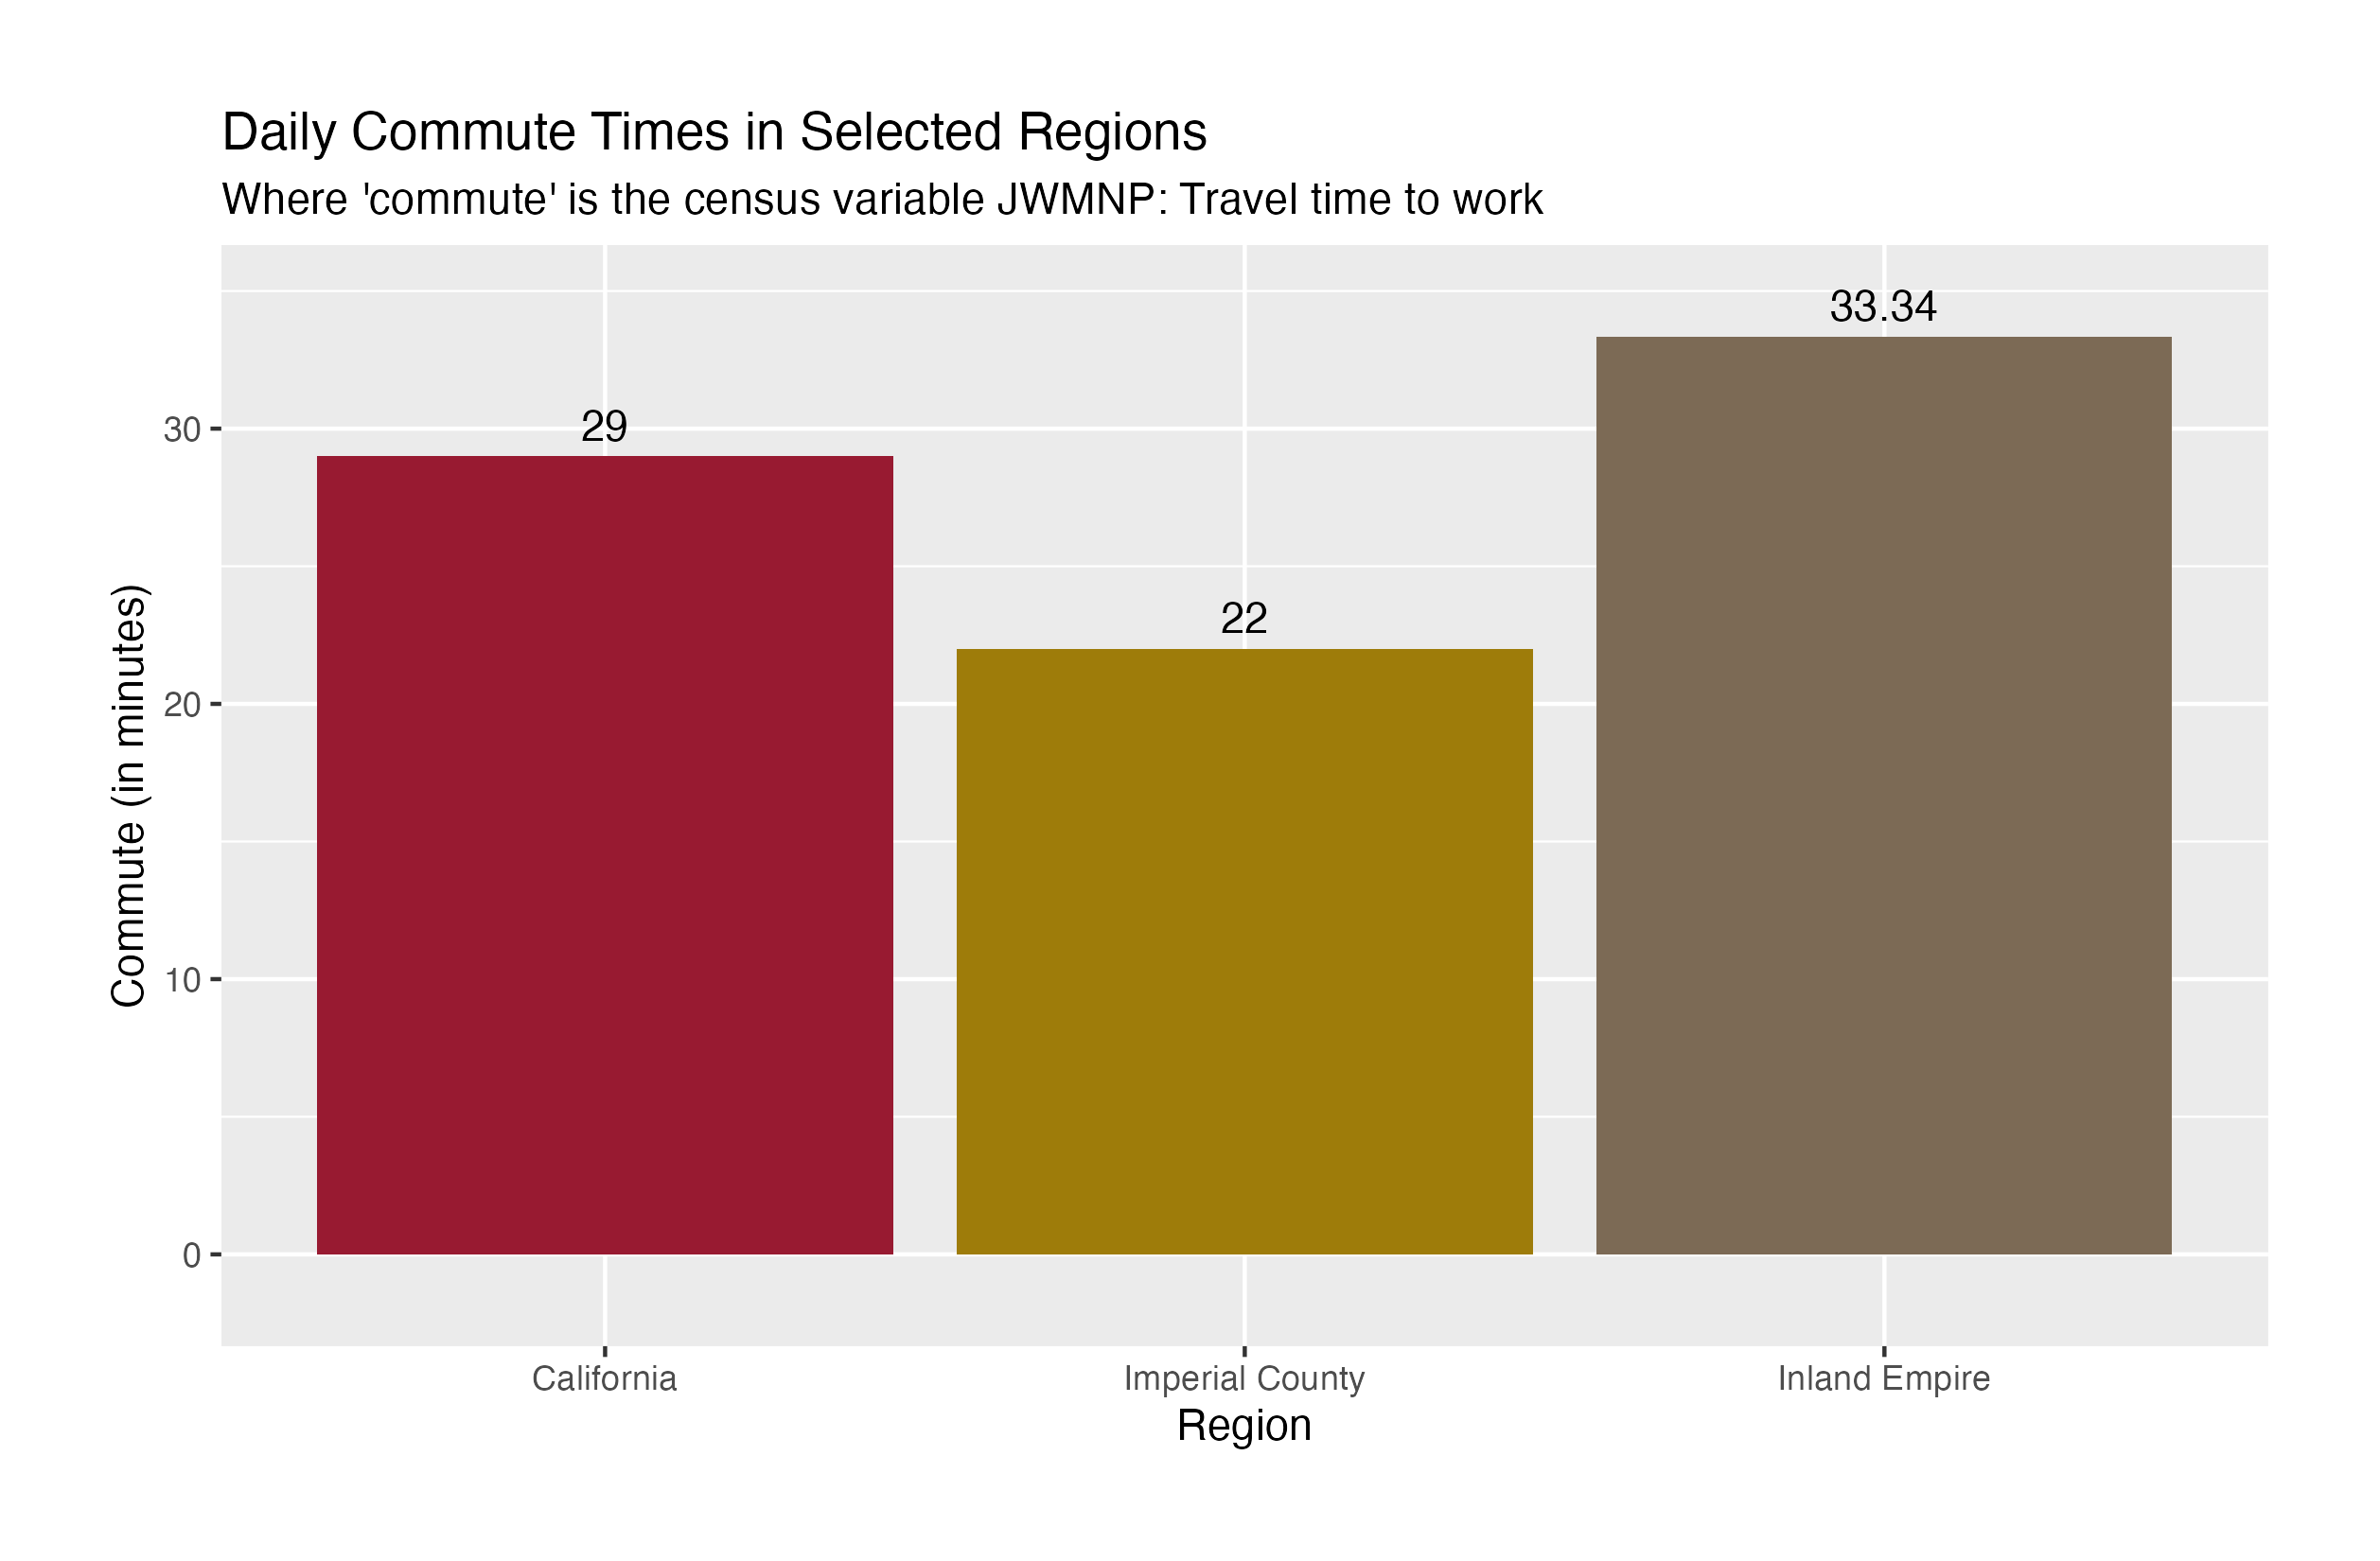
\includegraphics[width=\textwidth]{../IE-Employment/loweCommute.png}

\begin{itemize}
	\item The above graph illustrates the average daily travel time to work for California, Imperial County, and the Inland Empire in minutes.
	\item Notably, the commute for Inland Empire residents is roughly $50\%$ higher than that of Imperial county and roughly $15\%$ higher than typical Californians, indicating that IE residents are more likley to commute further. Given the Inland Empire's proximity to the country's second highest GDP MSA, Los Angeles-Long Beach-Anaheim, residents of the IE have abundant career opportunities both inside and outside their MSA. 
	\item Conversely, Imperial County's typical commute is rougly $25\%$ shorter than that of the typical Californian's, indicating that residents' job opportunities lie close to home. This is evidenced by Imperial County's remote location, as its major city, El Centro, lies roughly 113 miles away from San Diego, its closest major American city, meaning that residents are essentially confined to working in the sparsely-populated region. Although it is close to the Mexican city Mexicali, workers would need visa sponsorship to work legally in the city and would likely work for a considerably lower wage. 
\end{itemize}

\subsubsection*{Figure 2. Job Opportunity Index in Commutable Regions}
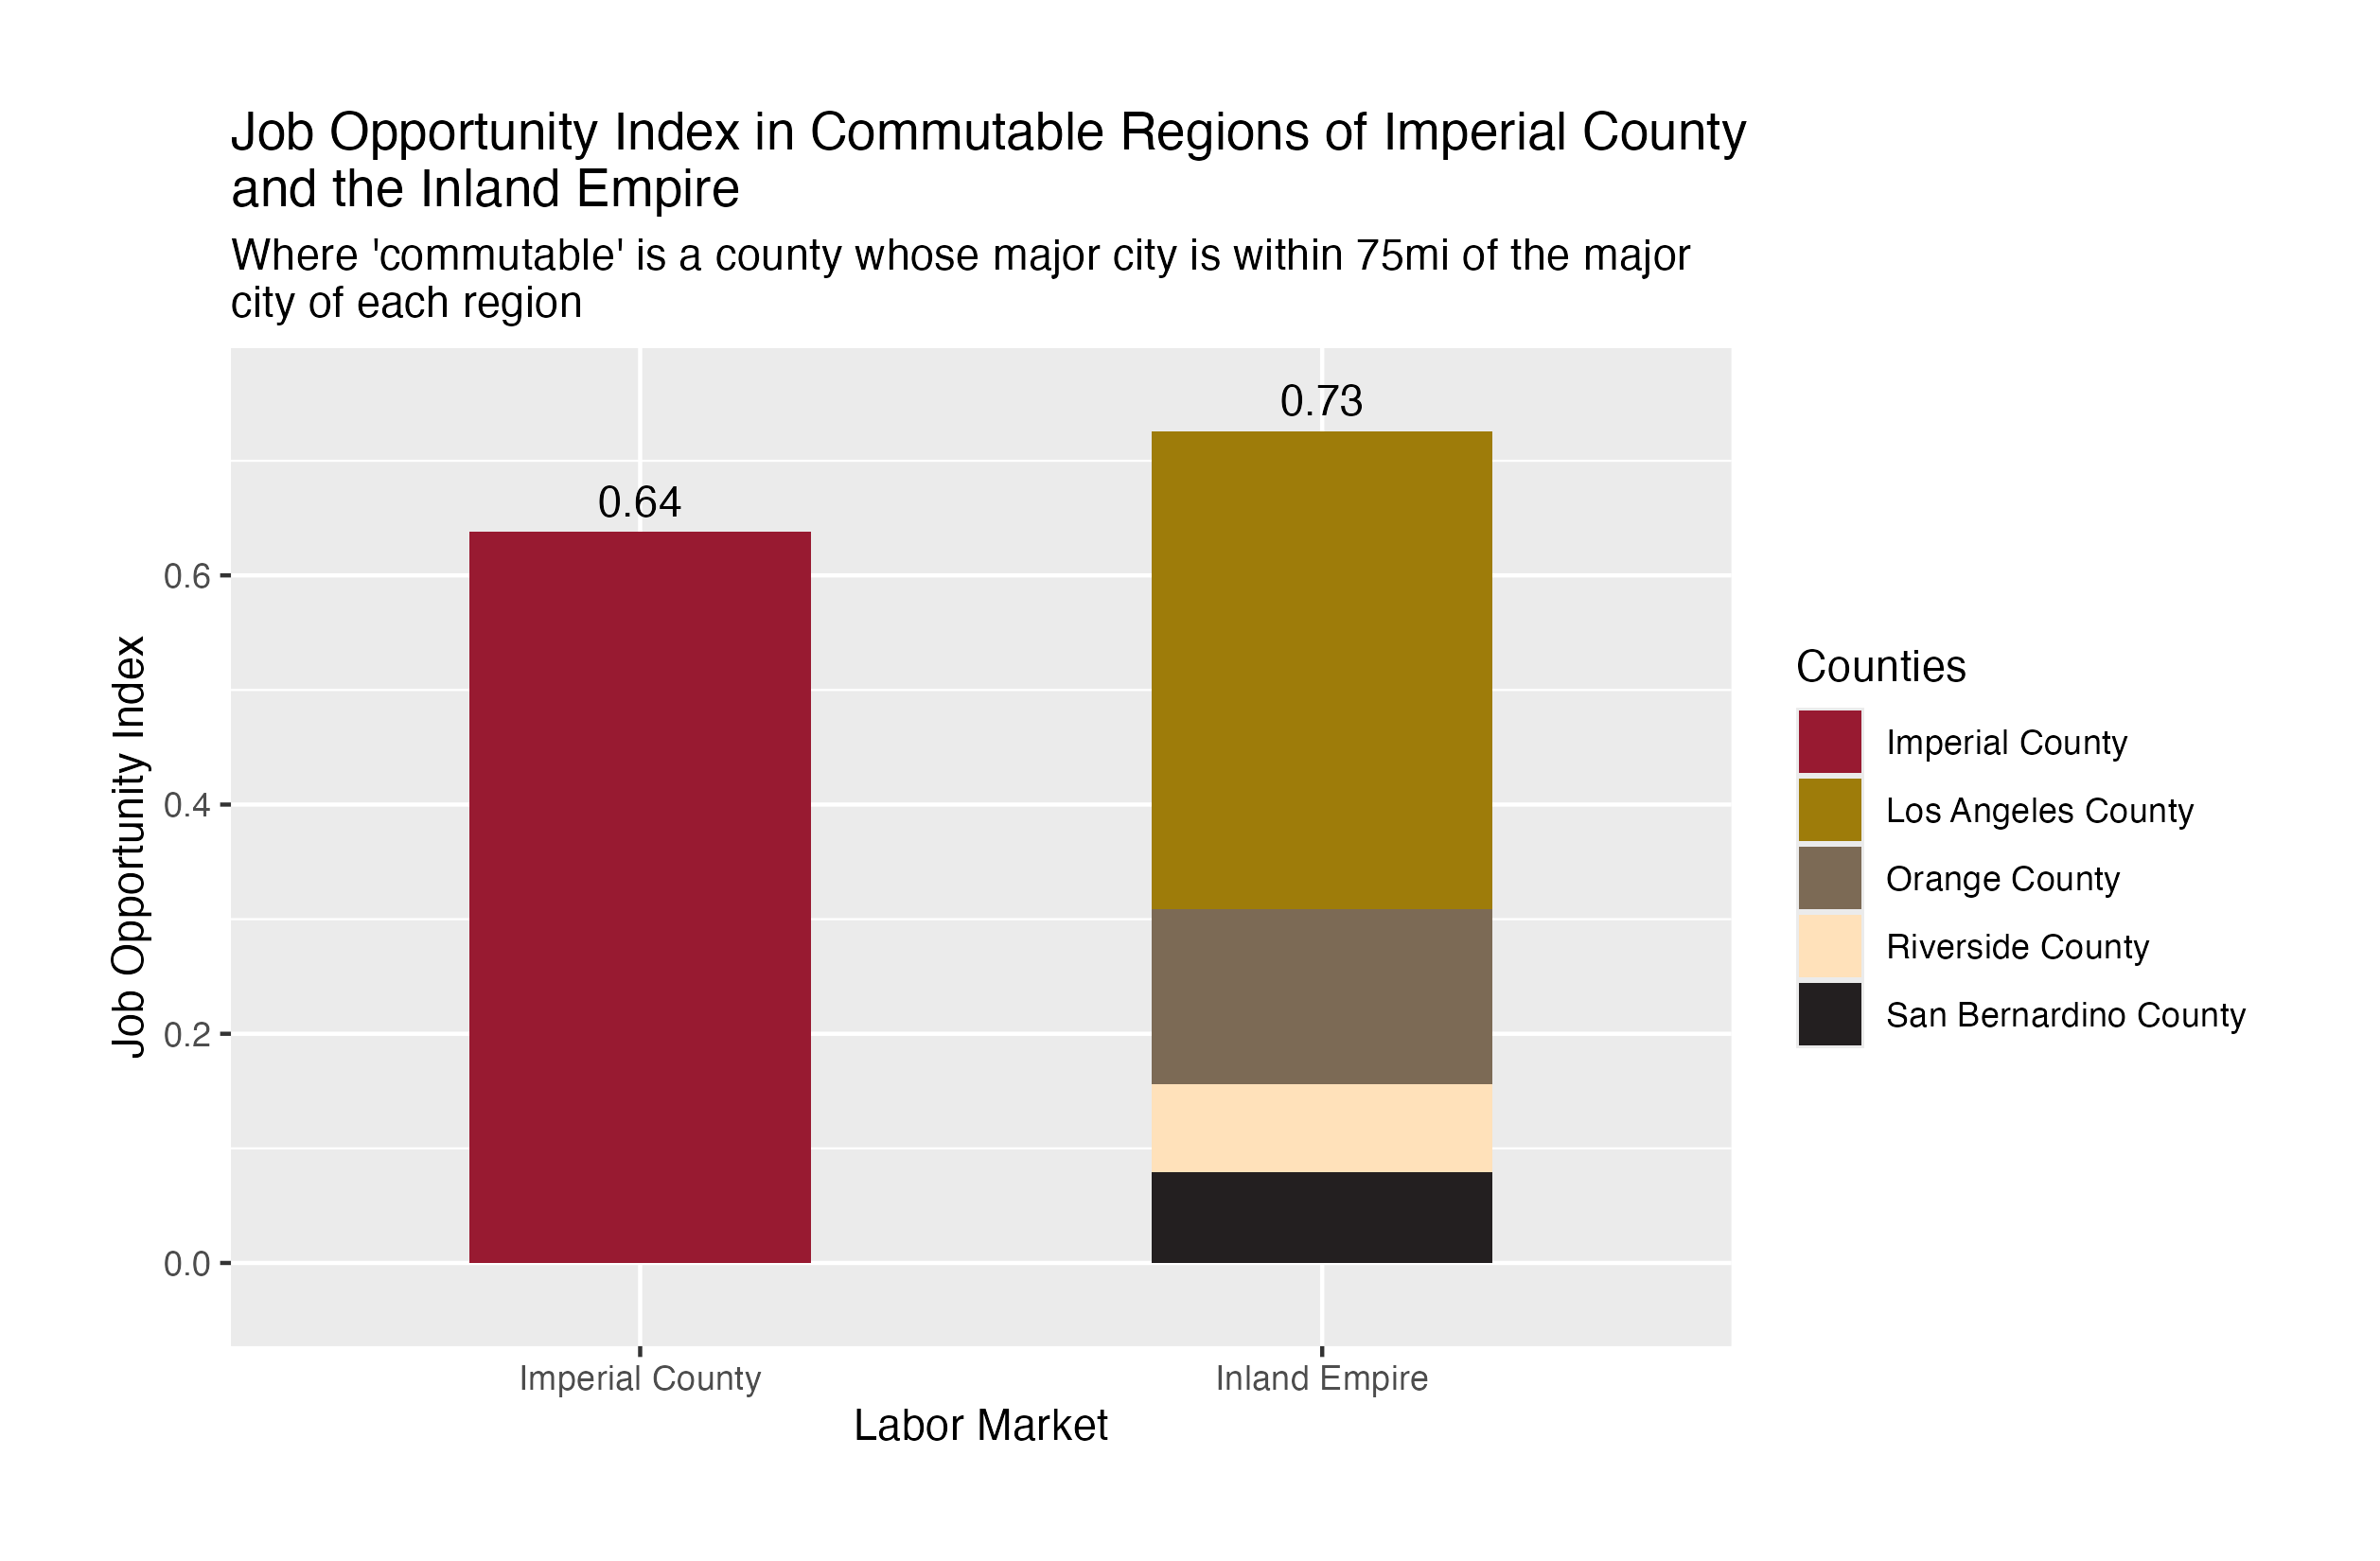
\includegraphics[width=\textwidth]{../IE-Employment/loweJOI.png}

\begin{itemize}
	\item The above graph illustrates the Job Opportunity Index (JOI), which intends to assess the accessibility of employment in a region, between Imperial County and the Inland Empire.
    \item The JOI is calculated as the ratio between the presence of jobs and the number of working-age people (which we use instead of labor force as an attempt to account for discouraged workers), in regions that are commutable from each labor market. We define "commutable" as being a county whose major city lies within 75 miles of the major city of the commuter's region. Imperial County had no commutable regions aside from its own, whereas the Inland Empire (San Bernardino and Riverside Counties) was commutable to both Los Angeles County and Orange County.
	\item Using the JOI metric, we find that jobs are roughly $14\%$ more accessible in the Inland Empire than they are in Imperial County. 
\end{itemize}

\subsubsection*{Elaboration}
The stark difference in unemployment rates between Imperial County and the Inland Empire (IE) stems from several sources, with geography playing a significant role. Imperial's remote location and distance from California's economic powerhouses limit residents' job opportunities—a sharp contrast to the convenient access enjoyed by those in the Inland Empire.

Additionally, Imperial County's predominantly rural character confines most of its economic activity to agriculture, leading to significant seasonal unemployment. Although the IE also has a strong farming sector, workers have more opportunities to find employment, as illustrated by the JOI comparison.

Finally, Imperial County's isolation makes it challenging to support California's high minimum wage, leading to fewer employment opportunities. While the IE's economy is deeply intertwined with the high-income Los Angeles metroplex, Imperial County relies heavily on its own smaller economy, meaning it cannot support as many workers, which leads to higher unemployment.

\subsection*{Sources}
\subsubsection*{Figure 1}
ACS 5-Year Estimates Public Use Microdata Sample (2023)

\subsubsection*{Figure 2}
DP05 - ACS Demographic and Housing Estimates (2024)
California Open Data Portal - Current Employment Statistics (CES)
Google Maps

\subsection*{Repository}
https://github.com/juhidamley/IE-Employment
\end{document}